\documentclass[../main.tex]{subfiles}

\begin{document}

\subsection{Physiopy - Documentation of Physiological Signal Best Practices}\label{sec:physiopy}

\authors{Sarah E. Goodale, %
Ines Esteves, %
Roza G. Bayrak, %
Neville Magielse, %
Stefano Moia, %
Yu-Fang Yang, %
The Physiopy Community}

\begin{figure*}
	\centering
	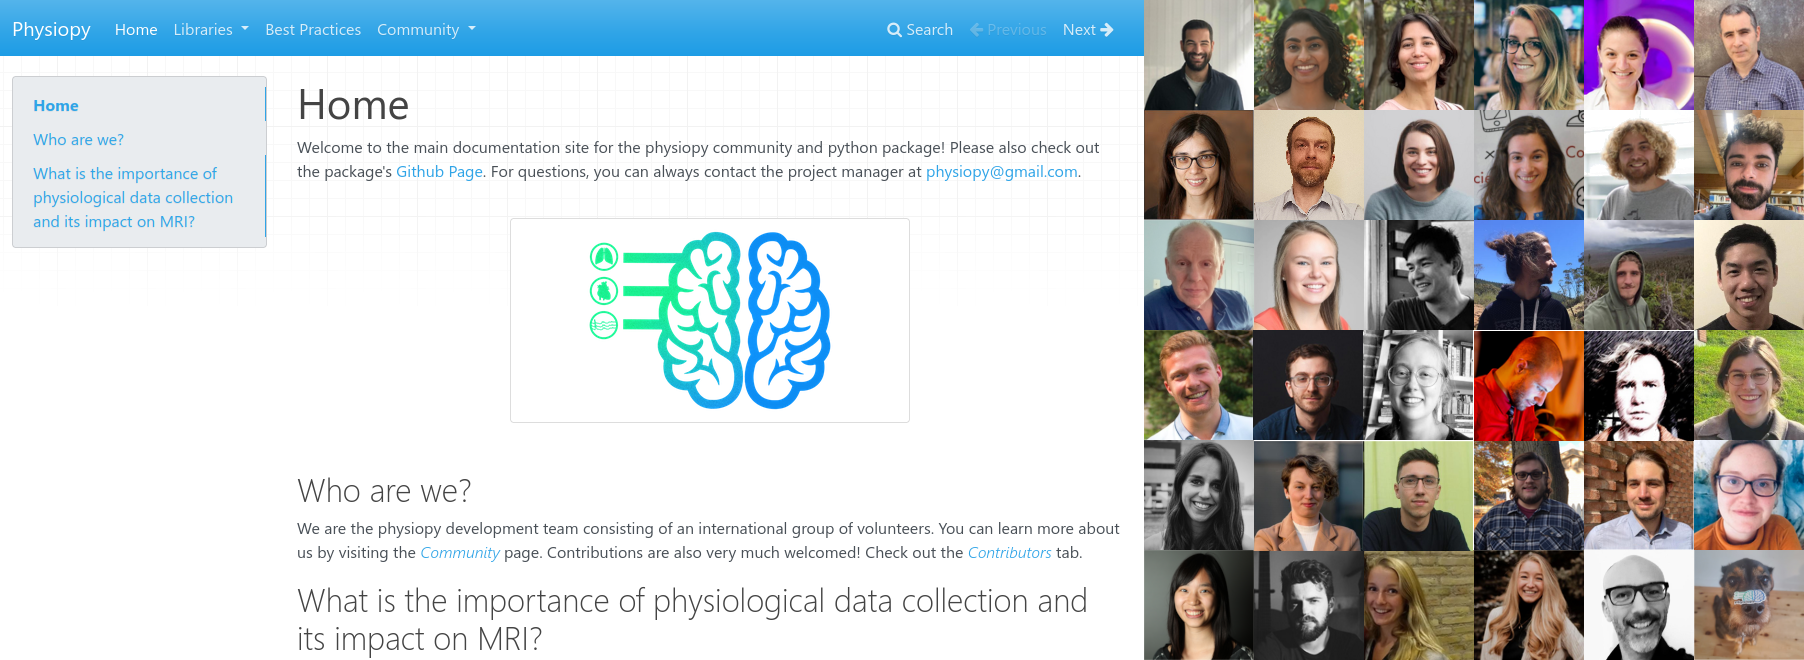
\includegraphics[width=1\textwidth]{physiopy-documentation_figure.png}
	\caption{Left: Current version of the documentation homepage; Right: Physiopy Contributors}
	% Add a label to reference in text. Make it specific!
	\label{fig:physiopy_beforeafter}
\end{figure*}

Physiological data provides a representation of a subject’s internal state with respect to peripheral measures (i.e., heart rate, respiratory rate, etc.). Recording physiological measures is key to gain understanding of sources of signal variance in neuroimaging data that arise from outside of the brain\citep{chen2020}. This has been particularly useful for functional magnetic resonance imaging (fMRI) research, improving fMRI time-series model accuracy, while also improving real-time methods to monitor subjects during scanning\citep{bulte2017, caballero-gaudes2017}. 

Physiopy (\url{https://github.com/physiopy}) is an open and collaborative community, formed around the promotion of physiological data collection and incorporation in neuroimaging studies. Physiopy is focused on two main objectives. The first is the community-based development of tools for fMRI-based physiological processing. At the moment, there are three toolboxes: \textit{phys2bids} (physiological data storage and conversion to BIDS format\citep{phys2bids}, \textit{peakdet} (physiological data processing), and \textit{phys2denoise} (fMRI denoising). The second objective is advancing the general knowledge of physiological data collection in fMRI by hosting open sessions to discuss best practices of physiological data acquisition, preprocessing, and analysis, and promoting community involvement. Physiopy maintains documentation with best practices guidelines stemming from these joint discussions and recent literature.

At the OHBM 2022 Brainhack, we aimed to improve our community documentation by expanding on best practices documentation, and gathering libraries of complementary open source software. This provides new users resources for learning about the process of physiological collection as well as links to already available resources.The short-term goal for the Brainhack was to prepare a common platform (and home) for our documentation and repositories. We prioritised fundamental upkeep and content expansion, adopting Markdown documents and GitHub hosting to minimise barriers for new contributors. Over the course of the Brainhack, and with the joint effort within three hubs (Glasgow, EMEA and Americas), we were able to improve the current community website by rethinking its structure and adding fundamental content relative to who we are, contributions, and updated best practices, such as creating home pages, easy to find and navigate contribution tabs, adding new information from community best practices discussions as well as links to relevant software and datasets. Additionally, we  aggregated the information scattered across different repositories, allowing important information for both the community and new collaborators to be accessible in a single location. 

The long-term goals of the community are to develop and sustain knowledge and instruments for physiological signal adoption in f/MRI settings. Our aim is to facilitate the coming-together of researchers that are just starting to include physiological measures and experienced users. This community will then provide consensus guidelines for standardised data collection and preprocessing. Building on what we have already achieved, we will continue to promote and document best practices. Further development is ongoing and anyone that is interested in physiological signal collection for f/MRI data, independently of their level and type of expertise, is highly encouraged to check Physiopy out, to join the community, or to contribute in any way.




\end{document}
